% Created 2024-02-15 Thu 20:04
% Intended LaTeX compiler: pdflatex
\documentclass[11pt]{article}
\usepackage[utf8]{inputenc}
\usepackage[T1]{fontenc}
\usepackage{graphicx}
\usepackage{longtable}
\usepackage{wrapfig}
\usepackage{rotating}
\usepackage[normalem]{ulem}
\usepackage{amsmath}
\usepackage{amssymb}
\usepackage{capt-of}
\usepackage{hyperref}
\author{Wei Wang}
\date{\today}
\title{Classical Guitar Lesson Handout}
\hypersetup{
 pdfauthor={Wei Wang},
 pdftitle={Classical Guitar Lesson Handout},
 pdfkeywords={},
 pdfsubject={},
 pdfcreator={Emacs 29.1 (Org mode 9.7)}, 
 pdflang={English}}
\begin{document}

\maketitle
\section*{Lesson 1}
\label{sec:org4a9f57e}
\subsection*{Assessments}
\label{sec:org014ff87}
\begin{center}
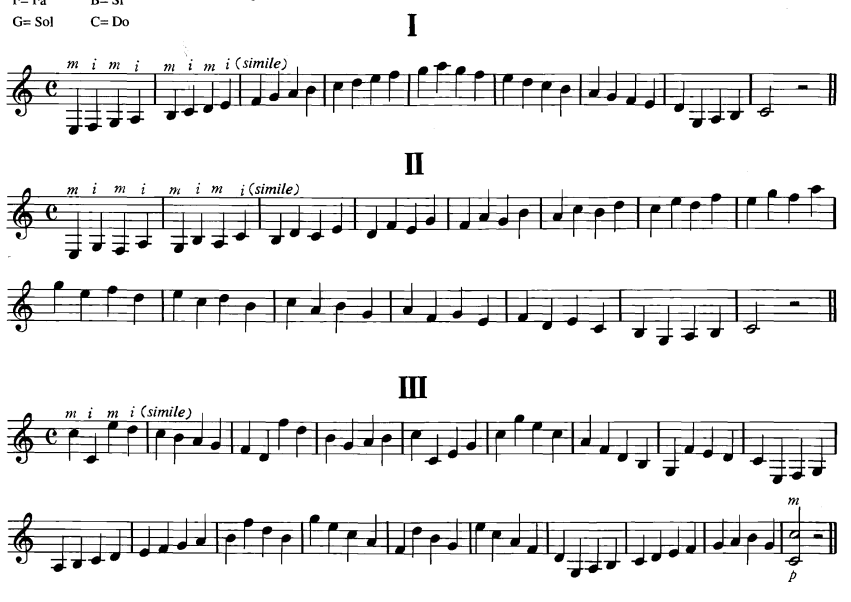
\includegraphics[width=.9\linewidth]{./Handouts.org_20240214_221205.png}
\end{center}
\subsection*{How to sit and hold your guitar}
\label{sec:orgb180b29}
\subsubsection*{How to sit}
\label{sec:org951b376}
\begin{itemize}
\item Sit on the front half of a chair, use a footstool for left foot
\item Be comfortable and relax
\item Four points of contact of the body
\end{itemize}
\begin{center}
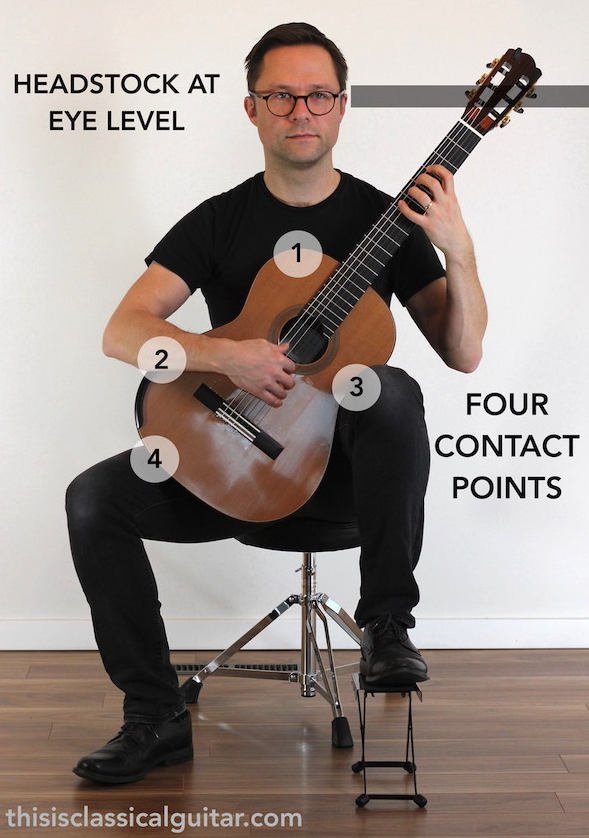
\includegraphics[width=.9\linewidth]{./Handouts.org_20240214_210131.png}
\end{center}
\subsubsection*{Left hand}
\label{sec:org6c26be6}
\begin{itemize}
\item Your elbow and left arm should never be allowed to be rigid or stiff
\item Never bent your wrist too much!
\item Hand is C shape
\item The thumb of you LH has to be free to move
\item Thumb should be across from the index and/or middle fingers
\end{itemize}
\subsubsection*{How to look at your left hand}
\label{sec:orgee14996}
\begin{itemize}
\item Learn to trust your left hand in regards to which string you are on.
\item Do not look at the entire fretboard and your left hand
\end{itemize}
\begin{center}
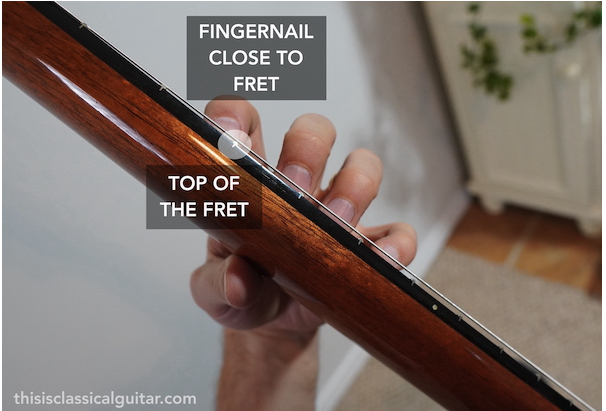
\includegraphics[width=.9\linewidth]{./Handouts.org_20240214_214427.png}
\end{center}
\subsubsection*{Position of the LH finger tips}
\label{sec:orga67f523}
\begin{itemize}
\item Try to ``stand'' on the fretboard
\item Play with finger tips, not pad
\item close to fret
\end{itemize}
\subsubsection*{Right hand}
\label{sec:org5fe5500}
\begin{itemize}
\item Nail shape, take care your nails (We will talk about this more in the future).
Start to keep 2-3 mm of nails on your right hand fingers
\item Straight wrist, in-line with your forearm
\item Relaxed arch
\item Use your hand in the way its designed, always grab naturally
\item Guitar position need to be correct to support correct RH
\end{itemize}
\subsection*{The Complete fretboard}
\label{sec:org5695760}
\begin{center}
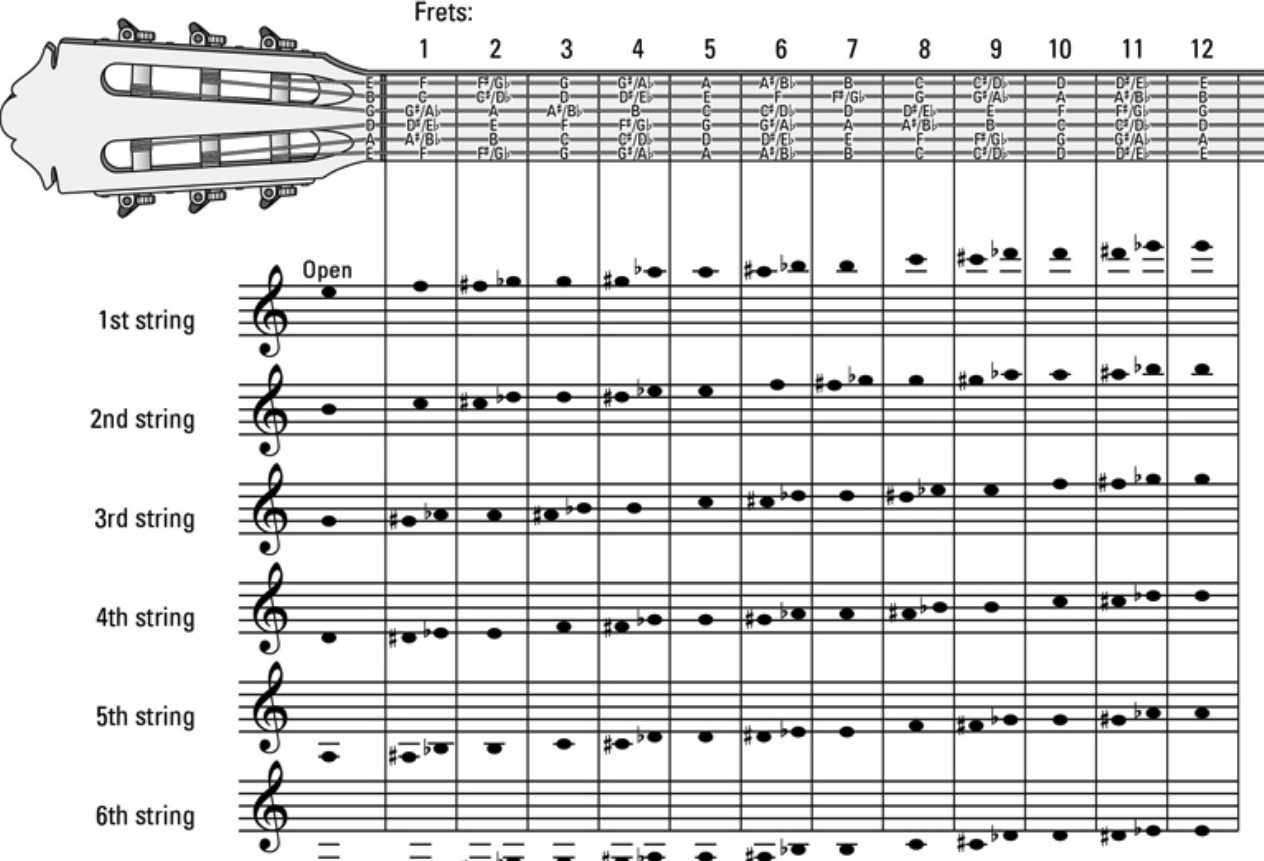
\includegraphics[width=.9\linewidth]{./Handouts.org_20240214_213412.png}
\end{center}
\subsection*{Music reading tips}
\label{sec:orgd193fd3}
\subsubsection*{The more references you have, the quicker you can read}
\label{sec:orgdadd7d3}
\begin{itemize}
\item Four spaces: FACE
\end{itemize}
\begin{center}
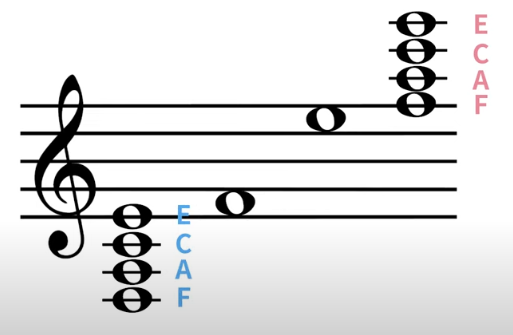
\includegraphics[width=.9\linewidth]{./Handouts.org_20240214_220600.png}
\end{center}
\begin{itemize}
\item GBD 搞不懂
\end{itemize}
\begin{center}
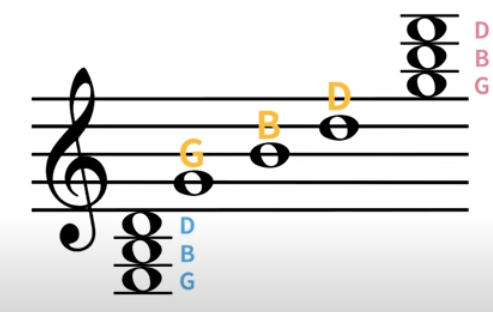
\includegraphics[width=.9\linewidth]{./Handouts.org_20240214_220721.png}
\end{center}
\subsection*{Exercises (with a metronome)}
\label{sec:orge033599}
\subsubsection*{Left hand exercise (2 fingers)}
\label{sec:org4b7889d}
\begin{itemize}
\item do it at a fret with ease (fret 5)
\begin{itemize}
\item finger 1 and finger 2
\item finger 2 and finger 3
\item finger 3 and finger 4
\item finger 1 and finger 3
\item finger 2 and finger 4
\item finger 1 and finger 4
\end{itemize}
\item watch for
\begin{itemize}
\item LH shape
\item minimize finger movement(don't left fingers too high)
\end{itemize}
\end{itemize}
\subsubsection*{Right hand exercise}
\label{sec:orgb24f0af}
\begin{itemize}
\item Page 18,
\begin{itemize}
\item Arpeggios with the thumb and three fingers
\item Pay attention to left finger
\begin{center}
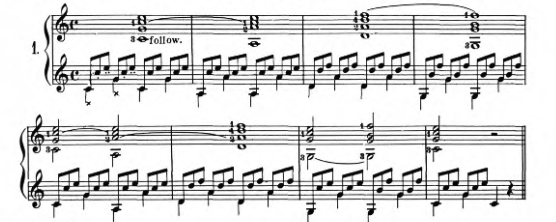
\includegraphics[width=.9\linewidth]{./Handouts.org_20240215_164708.png}
\end{center}
\end{itemize}
\end{itemize}
\subsubsection*{Chromatic scales at capo 0 position(if you are able to move higher, do it)}
\label{sec:org96f61ad}
\begin{itemize}
\item Use metronome!
\item Set tempo to 50, slowly increase to 60
\begin{itemize}
\item 1/4 notes
\item 1/8 notes (later)
\item 1/16 notes(later)
\end{itemize}
\end{itemize}
\subsubsection*{C Scales}
\label{sec:org4f3091b}
\begin{center}
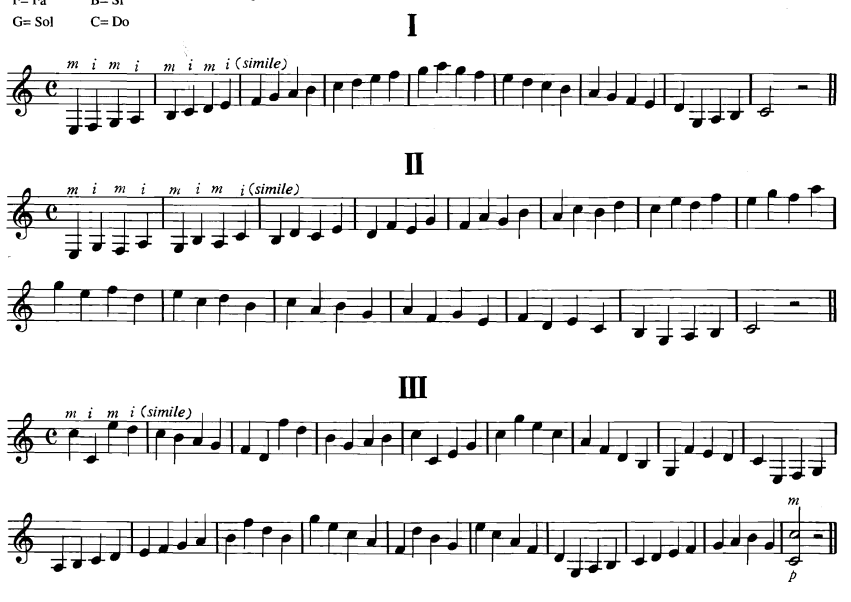
\includegraphics[width=.9\linewidth]{./Handouts.org_20240214_221205.png}
\end{center}
\subsubsection*{Arpeggios (broken chords)}
\label{sec:org825e41b}
\begin{center}
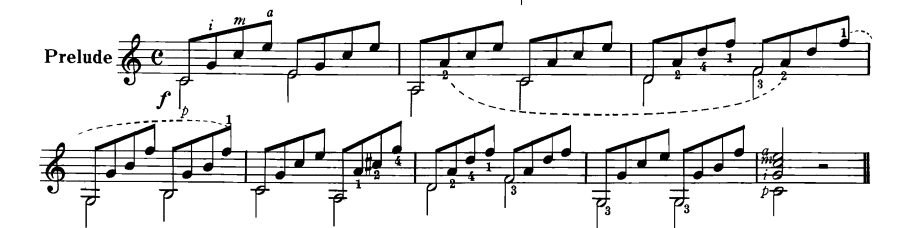
\includegraphics[width=.9\linewidth]{./Handouts.org_20240214_222243.png}
\end{center}
\subsection*{Music}
\label{sec:org954802b}
\subsubsection*{Andantino}
\label{sec:org592cfda}
\begin{center}
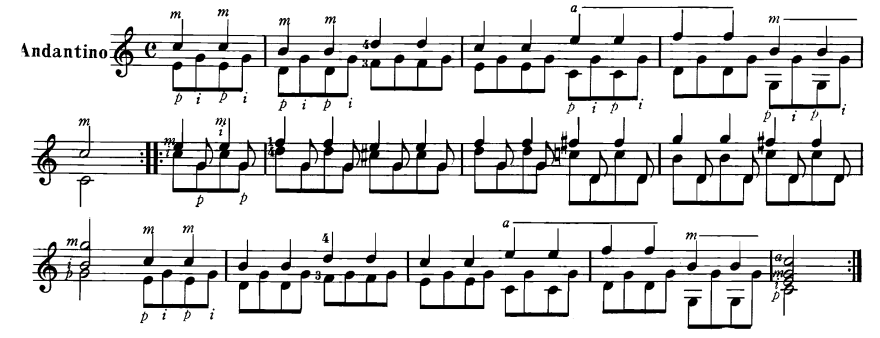
\includegraphics[width=.9\linewidth]{./Handouts.org_20240214_222412.png}
\end{center}
\subsubsection*{Waltz}
\label{sec:orgfd9a913}
\begin{center}
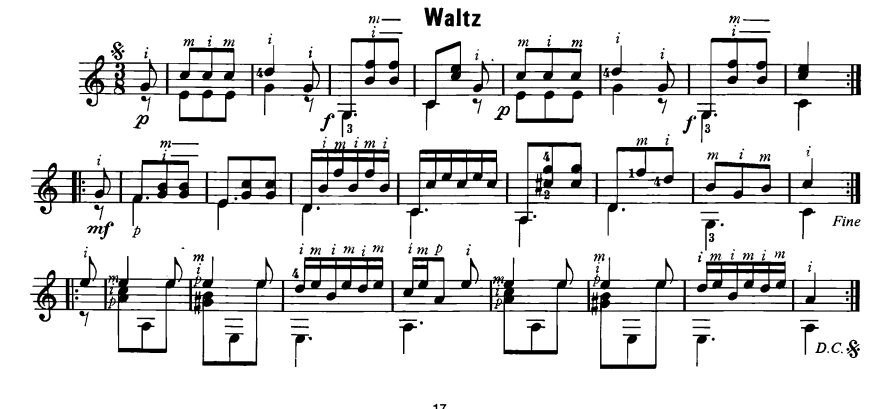
\includegraphics[width=.9\linewidth]{./Handouts.org_20240214_222357.png}
\end{center}
\subsection*{How to practice}
\label{sec:orge573f1a}
\begin{itemize}
\item 25 minutes daily
\item Prepare for the practice so you are interruption free(go to bathroom, get a glass of water near you, etc)
\item Find proper chair and use your footstool
\item Practice with a metronome
\item Practice SLOW, never practice with a tempo that you can't not control. Ask yourself
\begin{itemize}
\item Am I playing any wrong notes at this tempo?
\item Is my Rhythm 100\% correct?
\item How are my hand position?
\item Am I moving my fingers smoothly and freely?
\item Am I making beautiful sound?
\end{itemize}
\end{itemize}
\subsection*{What to practice}
\label{sec:org3f1739f}
\end{document}
